\chapter{Results}

\label{chap:results}

The experiments were conducted using the PostgreSQL 9.0.7 as the database system. Because of the nature of the advisor, all tests were performed on a single host from a cluster managed by OpenNebula 3.6. The host has one 2.4GHz dual core processor and 4GB RAM, running Fedora Linux 16, using kernel version 3.3.8. Even though the the library created to reallocate CPU in OpenRC should work with all the hypervisors supported by Libvirt, the experiments were only performed with KVM\footnote{http://www.linux-kvm.org/}. This hypervisor is already integrated within the mainline Linux kernel since the 2.6.0 kernel version. It was designed to support only hardware assisted virtualization.

For the tests performed during the calibration step, a special VM was created to be run on newly added hosts. It runs the Debian Squeeze Linux operating system, specially configured to be a database server. It contains a simple $300MB$ database, created with PGBench. Changes in the relational schema of the database are not very important for this step, as long as the query execution plans are known beforehand. For this reason, we do not need to go into further details on why a specific schema was chosen. Under the tested host, the VM was given both CPU cores and 2GB of RAM. Considering the database size, it was wholly loaded in memory. This decision does not have any impact on the results, since only the parameters that describe CPU should be calibrated, instead of I/O. The memory storage for PostgreSQL was created using standard features provided by the DBMS and Linux operating system. The PostgreSQL init scripts were modified to automatically handle this storage every time the database service is stopped or started, including the VM booting. As the calibration queries have a simple known query plan, the tuning parameters are only modified if their change has an effect on the query optimizer decisions.

All the other tests were performed using Transaction Processing Benchmark H (TPC-H) databases with scale factor $0.6$. When loaded into PostgreSQL with their indexes, the size of these databases is $4339 MB$.  The choice of this benchmark relies on the fact that \cite{Soror:2008:AVM:1376616.1376711} has a previous study on the nature of determined queries from this benchmark. We use this knowledge to create workloads with specific CPU needs during the experiments.  It was also decided that in order to minimize I/O effects, the databases should also be loaded  in a RAM based file system, even though they will not fit entirely in the available RAM. Each database runs in a VM with $1.8 GB$ of RAM.  Each virtual machine is assigned one virtual CPU, during the tests they are pinned to the same core. This magnifies the problem of CPU competition among VM guests, especially in our case, where the workloads are sequentially run. 

The sections included in this chapter follow a sequence similar to the one used in chapter ~\ref{chap:implementation}. They are used to show experiments used to test different parts of our solution. We start by showing results for the calibration phase, as it needs to be run before the advisor, in order to map resource allocation levels to tuning parameters. Then we show the results related to the execution of our advisor. The first experiment is conducted using static workloads ( i.e. workloads that do not have its CPU needs changed along execution ). It is used to test how effective is the configuration search from OpenRC. In the second experiment, small changes in the workload needs are performed to test how the online refinement step adjusts the cost model during execution. We finish with a third experiment, used to test the dynamic configuration management. Its objective is to observe how the advisor behaves to major changes in the workload.


\section{Calibration}

The parameters \textbf{cpu\_tuple\_cost} and \textbf{cpu\_operator\_cost} were calibrated using the query shown in subsection ~\ref{app:cal1}. The values obtained for different resource allocations are shown in figures ~\ref{fig:cpuop} and ~\ref{fig:cputp}, along with the linear regression performed on them. Based on these results, it is possible to observe that the parameters that describe CPU do not have a strict linear variation, as seen on  \cite{4401021}. However it contradicts  \cite{Soror:2008:AVM:1376616.1376711}, which affirmed that this variation was linear when the memory for the VM was allocated to $50\%$. Considering the linear equation to be
\[
 f(x) = m*x + b
\],
the asymptotic errors found were the following:
\begin{itemize}
 \item \textbf{cpu\_tuple\_cost}
 \begin{itemize}
  \item $m \approx 6,7\% $;
  \item $b \approx 3,9\% $;
 \end{itemize}
  \item \textbf{cpu\_operator\_cost}
 \begin{itemize}
  \item $m \approx 9.2\% $;
  \item $b \approx 5.6\% $.
 \end{itemize}
\end{itemize}

 
 \begin{figure}[ht]
 \centering
 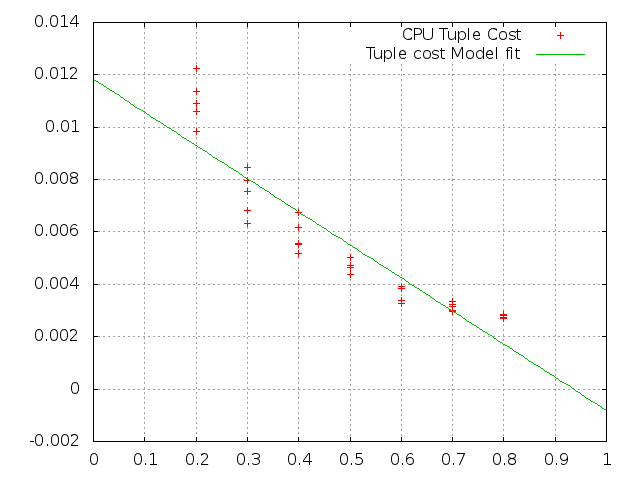
\includegraphics[width=0.8\textwidth]{cpu-operator-cost.png}
 \caption{Mapping of the $cpu\_operator\_cost$ parameter under different resource allocation levels during calibration}
 \label{fig:cpuop}
 \end{figure} 
% 
% 
 \begin{figure}[ht]
 \centering
 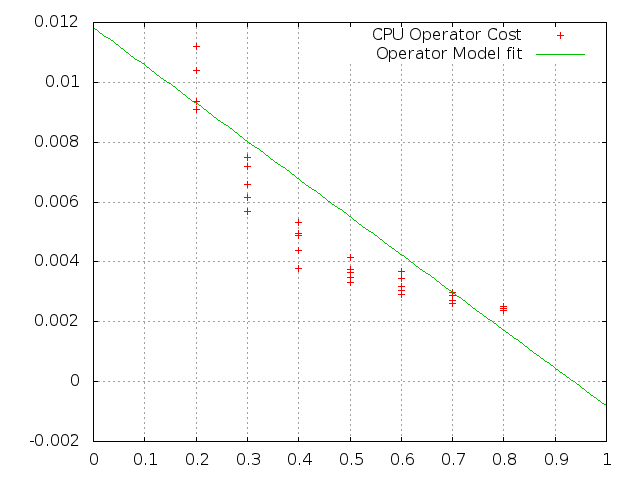
\includegraphics[width=0.8\textwidth]{cpu-tuple-cost.png}
 \caption{Mapping of the $cpu\_tuple\_cost$ parameter under different resource allocation levels during calibration}
 \label{fig:cputp}
 \end{figure} 
 
 The calibration of the parameter \textbf{cpu\_index\_tuple} was performed according to chapter ~\ref{chap:implementation}. The results were obtained through the execution of the query presented in subsection ~\ref{app:cal2}. They are shown in figure ~\ref{fig:cpuip}. The errors found for linear parameters $m$ and $b$ are approximately $8.6\%$ and $5.1\%$ , respectively.

 \begin{figure}[ht]
 \centering
 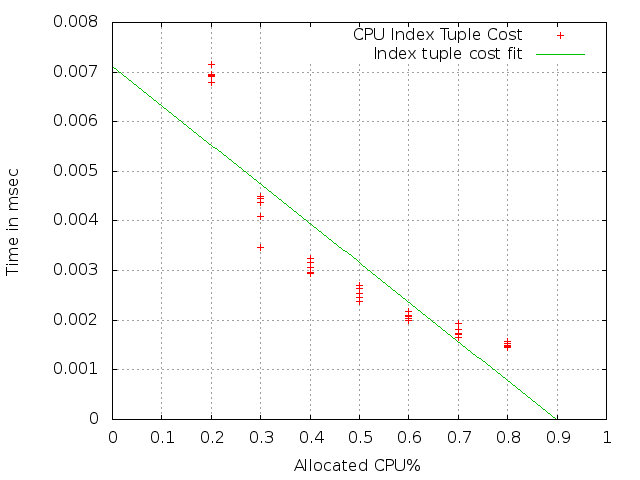
\includegraphics[width=0.8\textwidth]{cpu-index-tuple-cost.png}
 \caption{Mapping of the $cpu\_index\_tuple\_cost$ parameter under different resource allocation levels during calibration}
 \label{fig:cpuip}
 \end{figure} 
 
 \section{Advisor}
 

 
 To measure the performance of our advisor, we compare the costs of running the workloads under the recommended resource allocation to the default allocation. The default consists in simply allocating $1/N$ of the available CPU to the $N$ virtual machines. We consider $T_{default}$ and $T_{advisor}$ to be the execution time of the $N$ workloads running under the default resource allocation and the recommended one, respectively. The performance metric, defined in \cite{Soror:2008:AVM:1376616.1376711}, is the following:
 \[
  \frac{T_{default}-T_{advisor}}{T_{default}}
 \]
.
\subsection{Configuration Search}

In our first experiment, we show that the advisor can respond to different workload needs. Two TPC-H queries are used for this experiment, Q18 and Q21. In \cite{Soror:2008:AVM:1376616.1376711}, Q18 is described as one of the most CPU intensive queries. On the other hand, Q21 is one of the least CPU intensive queries, but it is much more I/O intensive than Q18. Based on these queries, two workload units are created. The first is the CPU-intensive workload unit, called C, which consists in instances of Q18. The second is the CPU non-intensive workload unit, called I, built with Q21 instances. Both of these units are scaled to have approximately the same execution time.

Based on these workload units, we create two workloads that are run by two different virtual machines. They are shown below:
\begin{eqnarray*}
 W_{1} &=& 5*C + 5*I \\
 W_{2} &=& k*C + (10-k)*I, 0 \leq k \leq 10. \\
\end{eqnarray*}
As $k$ increases, $W_{2}$ becomes more CPU intensive, while $W_{1}$ remains the same. The correct decision to be taken by our advisor as $k$ increases is to give $W_{2}$ more CPU. The results obtained are shown in figure ~\ref{fig:intensity}. For small $k$, the advisor is able to detect that $W_{2}$ is less CPU intensive, and most of the CPU allocation is given to $W_{1}$. The overall performance is improved  over the default allocation. As $k$ approaches $5$, the workloads become more alike. In this case, improvement is not possible. When $k$ is above $6$, new improvement  opportunities can be found by allocating more CPU to $W_{2}$. However the improvement is not at the same level as before, because both workloads are significantly CPU intensive. This means that the additional CPU allocation, given to $W_{2}$, causes a major performance decrease in $W_{1}$.

\begin{figure}[ht]
 \centering
 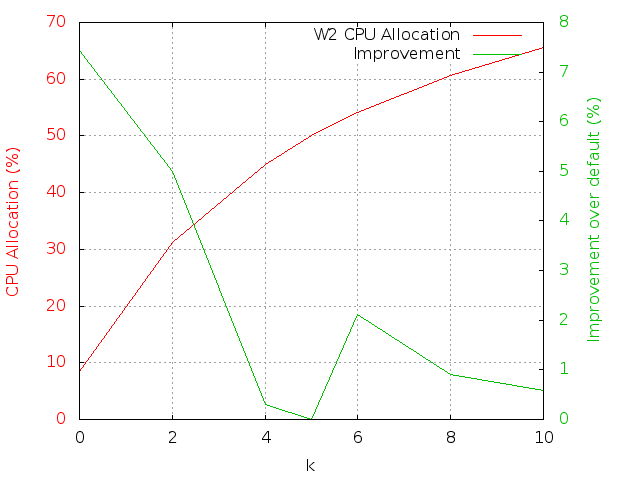
\includegraphics[width=0.8\textwidth]{improvement.png}
 \caption{Improvement achieved through configuration search for different CPU intensity levels}
 \label{fig:intensity}
\end{figure} 

The first experiment was also performed in \cite{Soror:2008:AVM:1376616.1376711} for two DBMSes, PostgreSQL 8.1.3 and DB2\footnote{http://www-01.ibm.com/software/data/db2/} V9.  The results obtained for PostgreSQL are significantly worse than those achieved in our implementation, specially for small $k$. They are shown in figure ~\ref{fig:cpuvar-psql}. The improvement rates found in \cite{Soror:2008:AVM:1376616.1376711} are generally below $2\%$. However, they are not very clear about where the TPC-H databases are loaded ( i.e. what type of file system and hardware was used ) and whether the I/O is proportionated among VMs or not. Furthermore, since they use Xen\footnote{http://www.xen.org/} as their hypervisor, they do not specify what type of virtualization technology they use. Xen supports both paravirtualization and hardware assisted virtualization. The virtualization choice affects the performance obtained during execution, although describing how the performance is affected is out of the scope of this 
paper.

\begin{figure}[ht]
 \centering
 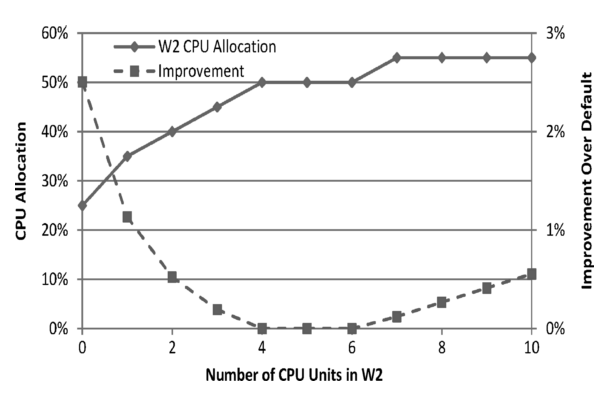
\includegraphics[width=0.8\textwidth]{CPU-var-psql.png}
 \caption{First experiment for PostgreSQL performed in \cite{Soror:2008:AVM:1376616.1376711}}
 \label{fig:cpuvar-psql}
\end{figure} 

\subsection{Online Refinement}

The objective of the online refinement is to correct errors in the cost estimator model. However, it also adapts the cost model to small changes in the workload. This means that there are two ways of testing this feature. The first is to run workloads for which the DBMS cost estimator has wrong estimates about. In this case, the errors need to be known beforehand. The second way of testing it is by analyzing how the advisor behaves for small changes in the workload. Using this second approach, we adapt the workloads presented in the first experiment in a second test. Although the online refinement was not disabled in the previous experiment, the workload did not change its needs along the execution. In this second experiment, we test the online refinement feature by modifying the workload along the execution. As $k$ increases, our advisor will try to adapt the model to these changes.

In this test $W_{1}$ and $W_{2}$ are defined as follows:
\begin{eqnarray*}
 W_{1} &=& 3*C + 2*I \\
 W_{2} &=& k*C + (5-k)*I, 0 \leq k \leq 2. \\
\end{eqnarray*}

We vary $k$ from $0$ to $2$ for $W_{2}$, while $W_{1}$ remains unchanged. Instead of comparing the results of the online refinement exclusively to the default allocation, we also compare it to the case in which only the initial configuration search is enabled. This way it is possible to analyze how disabling the online refinement and maintaining static decisions about the workloads may affect the overall performance. The results are shown in figure ~\ref{fig:online-ref-pf}. There it can be seen that without the online refinement, the performance is actually decreased. This happens because $W_{2}$ is treated as a CPU non-intensive workload all the time, thus its CPU needs are underestimated.
\begin{figure}[ht]
 \centering
 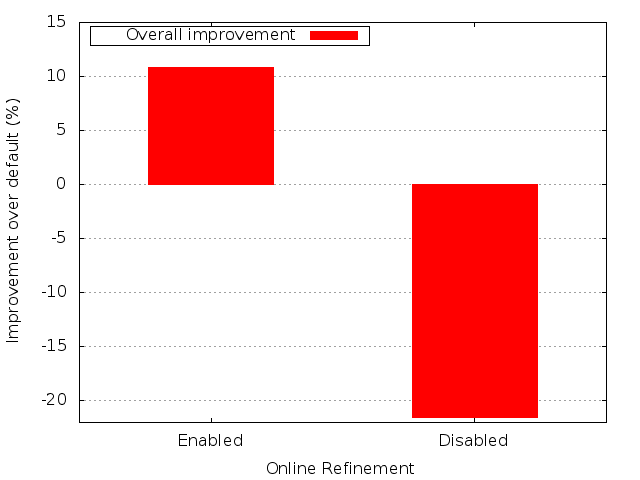
\includegraphics[width=0.8\textwidth]{online-ref.png}
 \caption{Online refinement effects on the improvement for the second experiment}
 \label{fig:online-ref-pf}
\end{figure} 

\subsection{Dynamic Configuration Management}

In OpenRC, this module is responsible for detecting major changes in the workload. In order to test it, it is necessary to cause abrupt changes in the workload needs. This way we are able to see how quickly the restart of the cost model can adjust our estimates. In this test, we compare two TPC-H workloads, called $W_{3}$ and $W_{4}$. Each one of them runs in separate virtual machines. Initially, $W_{3}$ more CPU intensive than $W_{4}$. At some point in execution, these workloads have their characteristics swapped ( i.e. $W_{4}$ becomes more CPU intensive than $W_{3}$ )

This experiment is run twice. At the first time, the dynamic configuration management is disabled. This means that we rely only on the online refinement for correcting the cost model. For the second run, we enable the detection for major workload changes. Our objective is to find out how faster we are able to achieve an optimal allocation by restarting the cost model from scratch.

The advisor is set up to monitor the workloads for changes at each $960$ seconds, and it will consider changes above $20\%$ in CPU needs as major changes. The workloads are split in several units. In figure ~\ref{fig:wkchanges}, we show the CPU allocation along the workload execution organized in periods. Each period defines a moment in which the configuration search was called. The class \textbf{DynamicConfigurationManagement} checks for workload changes just before the fourth period, while the actual swap in the workload needs starts happening after the third period. Once the workloads stabilize, the workload with high CPU needs should receive approximately $70\%$  of the available CPU. Here we show that by restarting the cost model, we can converge to the optimal value faster. At the fifth step of this experiment, $W_{3}$  was still considered less CPU intensive than $W_{4}$. This would incur in a much bigger problem for workloads that change frequently.

\begin{figure}[ht]
 \centering
 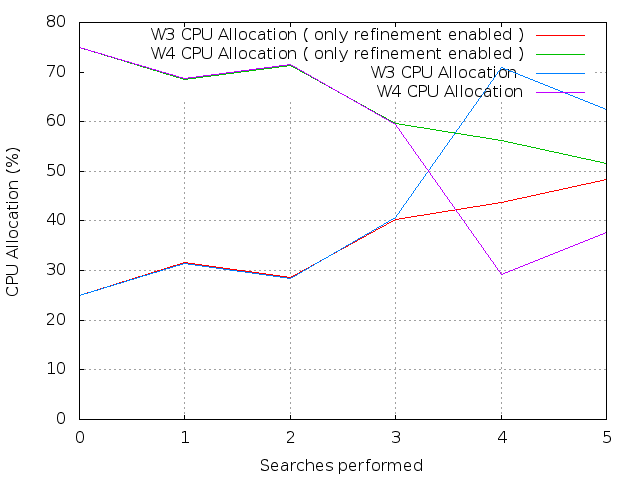
\includegraphics[width=0.8\textwidth]{dyn-change.png}
 \caption{Dynamic configuration management effects for the third experiment}
 \label{fig:wkchanges}
\end{figure} 


